\newcommand{\tikzI}{
	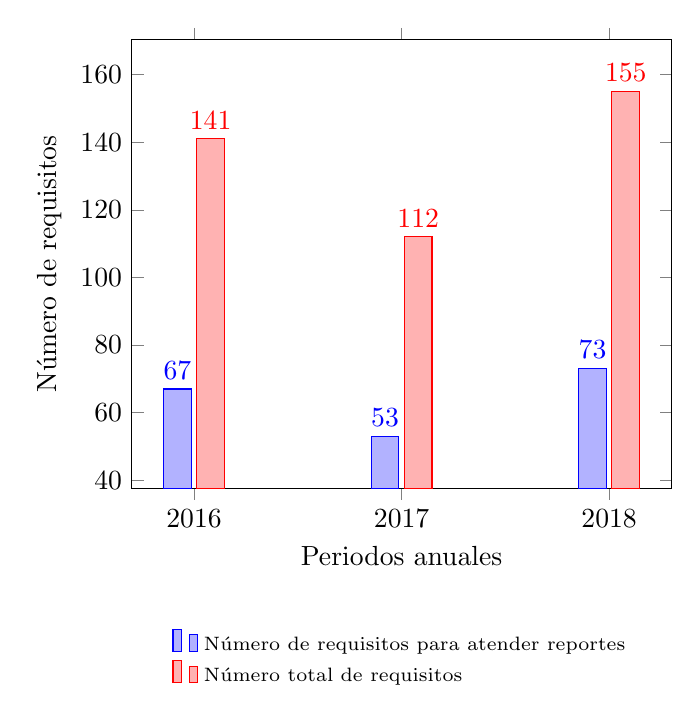
\begin{tikzpicture}
		\begin{axis}[
			ybar,
			enlargelimits=0.15,
			legend cell align={left},
			legend style={at={(0.5,-0.3)},
				anchor=north,legend columns=1, font=\scriptsize, draw=none},
			ylabel={N\'{u}mero de requisitos},
			symbolic x coords={2016,2017,2018},
			xtick=data,
			xlabel={Periodos anuales},
			nodes near coords,
			nodes near coords align={vertical},
			]
			\addplot coordinates {(2016,67) (2017,53) (2018,73)};
			\addplot coordinates {(2016,141) (2017,112) (2018,155)};
				\legend{
				N\'{u}mero de requisitos para atender reportes, 
				N\'{u}mero total de requisitos}
		\end{axis}
	\end{tikzpicture}
}